
\section{Shape of a dusty radiative bow wave}
\label{sec:shape-dust-wave}

As an alternative to hydrodynamic or magnetohydrodynamic bow shocks,
it is possible that some observed emission arcs may be bow waves due
to the action of radiation pressure on dust grains.

\begin{figure}
  \centering
  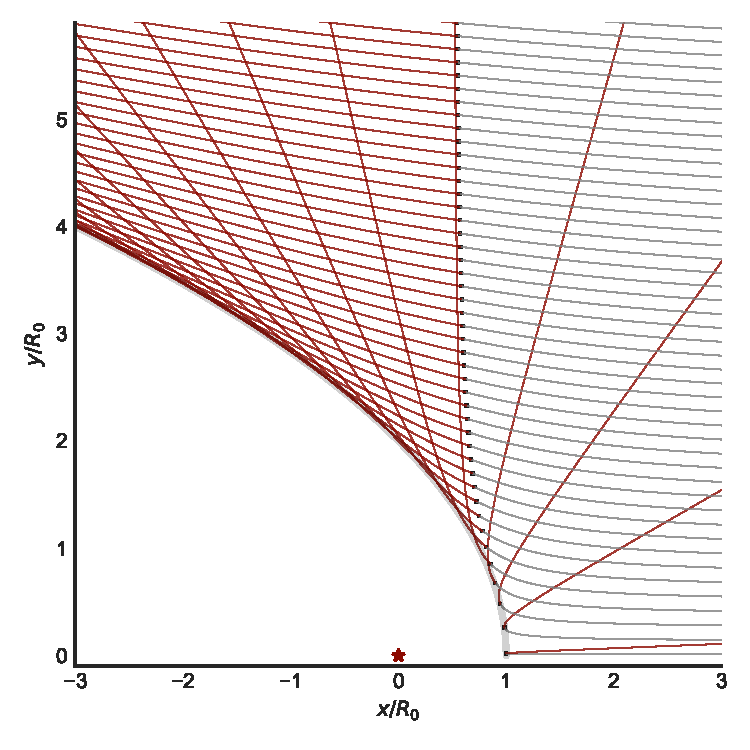
\includegraphics[width=\linewidth]{figs/dust-trajectories}
  \caption[Dust grain trajectories]{Dust grain trajectories under
    influence of a repulsive central \(r^{-2}\) radiative force.  Dust
    grains approach from the right at a uniform velocity and with a
    variety of impact parameters (initial \(y\)-coordinate). The
    central source is marked by a red star at the origin, and its
    radiative force deflects the trajectories into a hyperbolic shape,
    each of which reaches a minimum radius marked by a small black
    square.  The incoming hyperbolic trajectories are traced in gray
    and the outgoing trajectories are traced in red.  The locus of
    closest approach of the outgoing trajectories is parabolic in
    shape (traced by the thick, light gray line) and this constitutes
    the inner edge of the bow wave. }
  \label{fig:dust-trajectories}
\end{figure}



\newcommand\Qp{\ensuremath{Q_{\text{p}}}}
\newcommand{\grain}{\ensuremath{_{\text{d}}}}
\newcommand{\xsec}{\ensuremath{\sigma\grain}}
\newcommand\frad{\ensuremath{f_{\text{rad}}}}
\newcommand\thm{\ensuremath{\theta_{\text{m}}}}
A dust grain of geometrical cross-section \(\xsec\) situated a
distance \(R\) from a point source of radiation with luminosity \(L\)
will experience a repulsive, radially directed radiative force
\citep[e.g.,][]{Spitzer:1978a}
\begin{equation}
  \label{eq:dust-rad-force}
  \frad = \frac{\xsec \Qp L} {4 \pi R^2 c} e^{-\tau}
\end{equation}
where \Qp{} is the frequency-averaged\footnote{%
  Frequency averages of any quantity \(x\) should be understood as
  weighted by the attenuated source spectrum:
  \(\langle x \rangle_\nu = (L \, e^{-\tau})^{-1} \int_0^\infty x(\nu)\, L_\nu \, e^{-\tau_\nu} \, d\nu
  \).  } %
radiation pressure efficiency\footnote{%
  For absorption efficiency \(Q_{\text{abs}}\), scattering efficiency
  \(Q_{\text{scat}}\), and asymmetry parameter (mean scattering
  cosine) \(g\), we have
  \(\Qp = Q_{\text{abs}} + (1 - g) Q_{\text{scat}}\)
  \citep[e.g., \S~4.5 of][]{Bohren:1983a}.} %
of the grain, \(c\) is the speed of light, and \(\tau\) is the
frequency-averaged optical depth between the source and the grain.
For simplicity, we will consider only the optically thin case,
\(\tau \to 0\).

\subsection{Gas-free bow wave}
\label{sec:gas-free-bow}


If \(\frad\) is the only force experienced by the grain, then it will
move on a \textit{ballistic} trajectory, determined by its initial
speed at large distance, \(v_\infty\), and its impact parameter, \(b\).
For \(b = 0\), the grain radially approaches the source with initial
radial velocity \(-v_\infty\), which is decelerated to zero at the distance
of closest approach, \(R_0\), given by energy conservation:
\begin{equation}
  \label{eq:dust-r0}
  R_0 = \frac{\xsec \Qp L} {2 \pi c m\grain v_\infty^2} \ ,
\end{equation}
where \(m\grain\) is the grain mass.  The grain then turns round and
recedes from the source along the same radius, reaching a velocity of
\(+v_\infty\) at large distance.  For \(b > 0\), the trajectory,
\(R\grain(\theta; b)\), is found\footnote{%
  The problem is formally identical to that of Rutherford scattering,
  or (modulo a change of sign) planetary orbits.  The method of
  solution (via introduction of a centrifugal potential term and
  reduction to a 1-dimensional problem) can be found in any classical
  mechanics text \citep[e.g.,][\S~14]{Landau:1976a}.} %
to be hyperbolic, characterized by an eccentricity,
\(\varepsilon = \bigl( 1 + 4 b^2 / R_0^2\bigr)^{1/2}\), and polar angle of
closest approach, \(\thm = \cos^{-1} \varepsilon^{-1}\).  The trajectory is
symmetrical about \(\thm\) and can be written as
\begin{equation}
  \label{eq:dust-r-theta}
  \frac{R\grain(\theta; b)} {R_0} = 
  \frac{ \tfrac12 \bigl( \varepsilon^2 - 1 \bigr)} {\varepsilon \cos(\theta - \thm) - 1} \ , 
\end{equation}
with a total deflection angle of \(2 \thm\), which is equal to
\(90^\circ\) when \(b = 0.5 R_0\).  If the incoming dust grains initially
travel along parallel trajectories with varying \(b\), but the same
\(v_\infty\), then deflection by the radiative force will form a bow wave
around the radiation source, as shown in
Figure~\ref{fig:dust-trajectories}.  However, the inner edge of the
bow wave, \(R_{\text{in}}(\theta)\) is not given by the closest approach
along individual trajectories, \(R\grain(\thm; b)\), but instead must
found by minimizing \(R\grain(\theta; b)\) over all \(b\) for each value of
\(\theta\), which yields
\begin{equation}
  \label{eq:dust-r-in}
  \frac{R_{\text{in}}(\theta)} {R_0} = \frac{2}{1 + \cos\theta} \ .
\end{equation}
This is the polar form of the equation for the confocal parabola,
which we have already discussed in detail in \S~\ref{sec:conic} and
Appendix~\ref{app:parabola}.

The apex stagnation radius, \(R_0\), of the bow wave depends on the
grain properties via the combination \(\xsec \Qp / m\grain\).  For
grains of size \(a\grain\) and internal density \(\rho\grain\), we have
\(\xsec / m\grain \approx (a\grain \rho\grain)^{-1}\).  For radiation with
wavelength smaller than the grain size, \(\lambda < a\grain\), the
efficiency is \(\Qp \sim 1\), whereas for \(\lambda > a\grain\) it is
\(\Qp \sim a\grain/\lambda\).  Therefore, we would expect \(R_0\) to be almost
independent of grain size for small grains, but to vary as
\(R_0 \propto a\grain^{-1}\) for large grains, where small/large is relative
to the peak wavelength of the radiation source.  In principle, a
polydisperse population of grains could produce a blurring of the
observed bow wave, but only if large grains contribute significantly
to the dust emission.


\newcommand\drag{\ensuremath{_{\text{drag}}}}
\newcommand{\gas}{\ensuremath{_{\text{gas}}}}
\newcommand{\drift}{\ensuremath{_{\text{drift}}}}
\newcommand\soundspeed{\ensuremath{c_{\text{s,gas}}}}


\begin{figure}
  \centering
  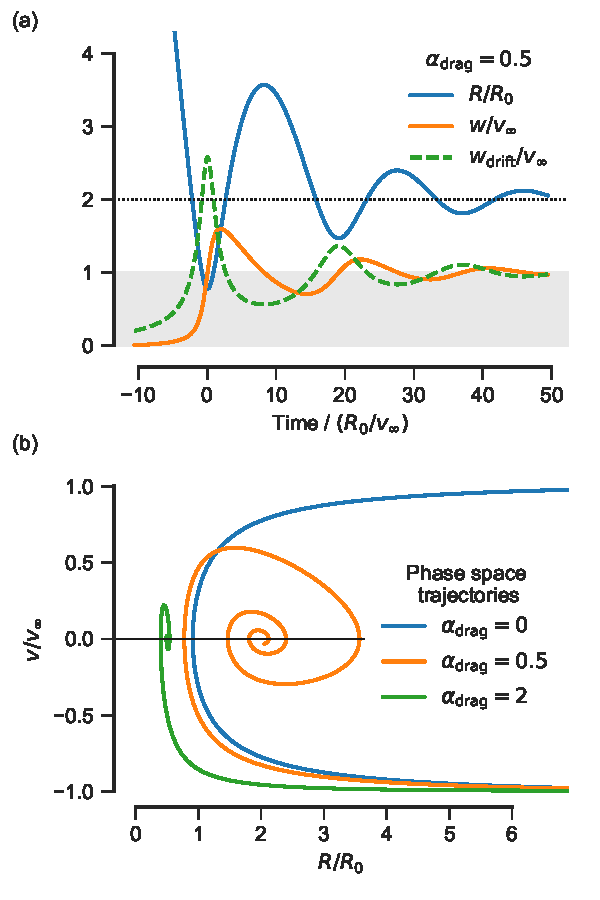
\includegraphics[width=\linewidth]{figs/dust-coupling-1d}
  \caption{Dust-gas coupling for an on-axis (purely radial)
    trajectory.  (a)~Grain radial position, \(R/R_0\), gas--grain
    velocity difference, \(w/v_\infty\), and local asymptotic drift
    velocity, \(w\drift/v_\infty\), versus time for
    \(\alpha\drag = 0.5\).  (b)~Phase space (position, velocity)
    trajectories for \(\alpha\drag = 0\), 0.5, and 2. For
    \(\alpha\drag > 0\), the grain spirals in on the point
    \((x, u) = (\alpha\drag^{-1}, 0)\).}
  \label{fig:dust-coupling-1d}
\end{figure}

\begin{figure*}
  \centering
  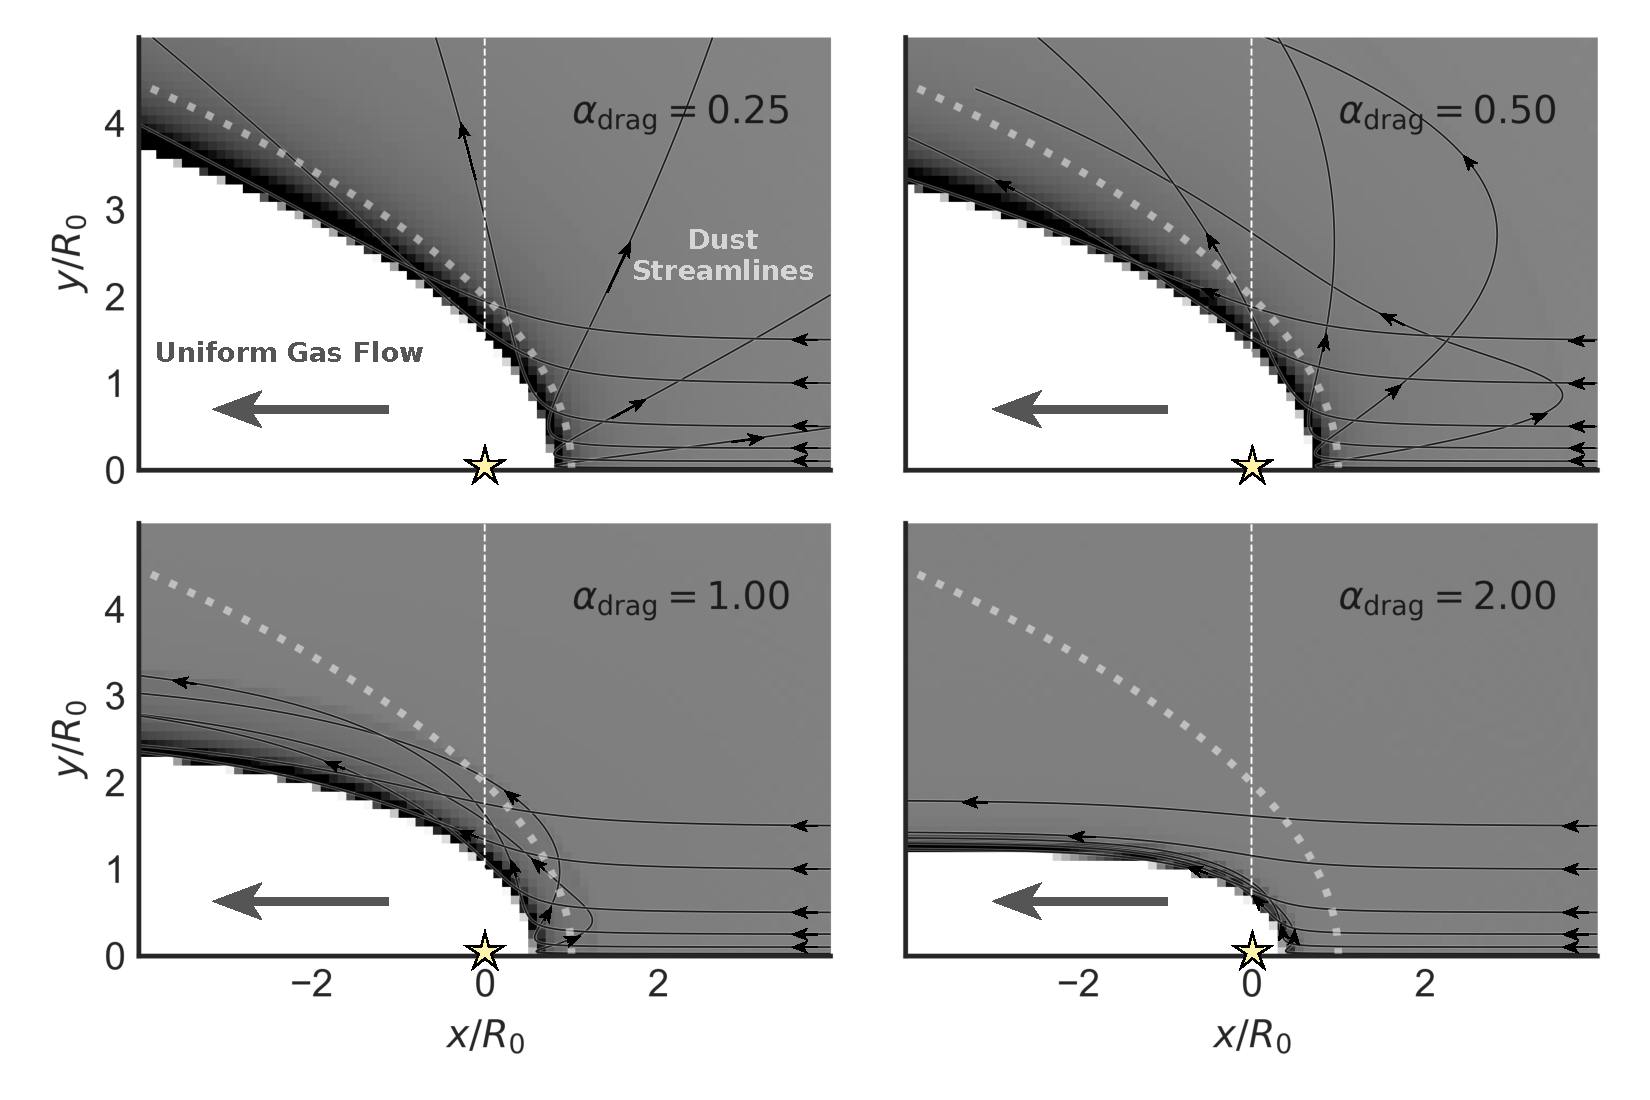
\includegraphics[width=\linewidth]{figs/dust-couple-stream-annotate}
  \caption{Dust grain trajectories under influence of gas drag in
    addition a repulsive central radiative force.  The dust
    streamlines are shown in blue and the dust density as a linear
    color scale, with maximum (white-yellow) of twice the ambient dust
    density.  Results are shown for four values of the drag parameter
    (see text): \(\alpha_\text{drag} = 0.25\), \(0.5\), \(1.0\), and
    \(2.0\). The shape of the bow wave for the drag-free case
    (Fig.~\ref{fig:dust-trajectories}) is shown by the thick dotted
    line.}
  \label{fig:dust-wave-coupling}
\end{figure*}


\subsection{Bow wave with gas drag}
\label{sec:bow-wave-drag}

More realistically, a grain will also be subject to a drag force,
\(f\drag\), due to its relative motion with respect to gas or plasma
particles. If the gas density, velocity, and sound speed are
\(\rho\gas\), \(v\gas\), and \(\soundspeed\), then a grain with velocity
\(v\grain\) will experience a drag force that is directed opposite to
the relative velocity, \(w = v\grain - v\gas\).  In the supersonic
limit, \(\abs{w} \gg \soundspeed\), the magnitude of the force is
\begin{equation}
  \label{eq:dust-fdrag}
  \abs{f\drag} \approx Q\drag \xsec \rho\gas w^2 \ ,
\end{equation}
where \(Q\drag\) is a boost factor to account for the increase in
cross section due to the Coulomb force when a charged grain interacts
with an ionized plasma \citep{Draine:1979a}.  We neglect the back
reaction of the dust on the gas motion and assume a uniform background
gas flow with \(v\gas = -v_\infty\).



Considering the incoming flow on the symmetry axis, at each radius
there is an asymptotic gas--grain drift speed, \(w\drift\), for which
the radiative and drag forces exactly cancel, \(f\drag = -\frad\),
yielding
\begin{equation}
  \label{eq:dust-wdrift}
  w\drift = \left( \frac{\Qp L} {4\pi c Q\drag \rho\gas R^2} \right)^{1/2} \ .
\end{equation}
Any deviation of \(w\) from \(w\drift\) produces unbalanced forces
that tend to restore \(w \to w\drift\).  We define a dimensionless
coupling coefficient, \(\alpha\drag\), to be the speed of the incoming
stream in units of the drift velocity at the radiative stagnation
radius:
\begin{equation}
  \label{eq:dust-alpha}
  \alpha\drag \equiv \frac{v_\infty} {w\drift(R_0)} = \left(
    Q\drag \frac{R_0 / a\grain} {\rho\grain / \rho\gas}
  \right)^{1/2} \ ,
\end{equation}
where we have used equation~\eqref{eq:dust-r0} and suppressed a
grain-shape dependent geometric factor of order unity.  If
\(\alpha\drag \ll 1\), then \(w\drift \gg v_\infty\) out to several times the
stagnation radius, so the radiation field has no difficulty in
effectively decoupling the grain from the gas and producing the
velocity difference, \(w = 2 v_\infty\), that is required to turn the grain
around and expel it towards the direction whence it came.  However,
for non-zero \(\alpha\drag\) the \(R^{-1}\) dependence of \(w\drift\)
(eq.~\eqref{eq:dust-wdrift}) means that the grain will
\textit{re-couple} to the inflowing gas stream around a radius
\(\approx R_0 / \alpha\drag \) and be swept in again for another try.  A further
effect of increasing \(\alpha\drag\) is that the grain penetrates closer to
the star on its initial approach, thanks to the tail wind provided by
the gas flow.  Both these behaviors are illustrated in
Figure~\ref{fig:dust-coupling-1d}, where it can be seen that the grain
inertia means that \(w\) lags behind the changes in \(w\drift\) and
the phase space trajectory is spiral, converging on the point
\((R, v) = (R_0 / \alpha\drag, 0)\).



\begin{figure}
  \centering
  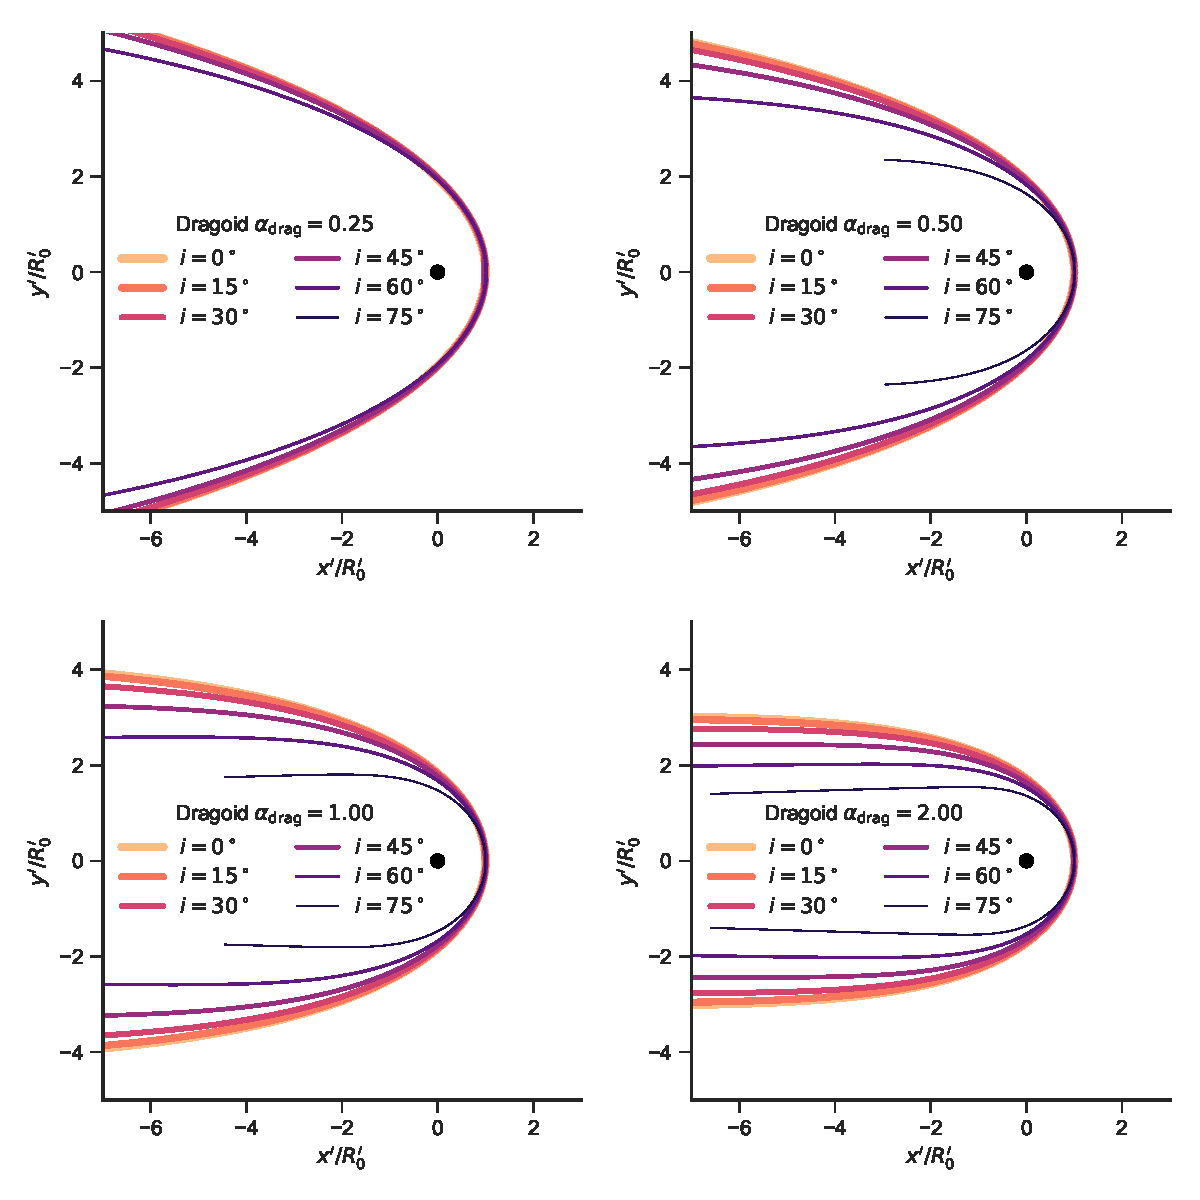
\includegraphics[width=\linewidth]{figs/test_xyprime_dragoid}
  \caption{Plane-of-sky shapes for dragoids.}
  \label{fig:dragoid-xy-prime}
\end{figure}


\begin{figure}
  \centering
  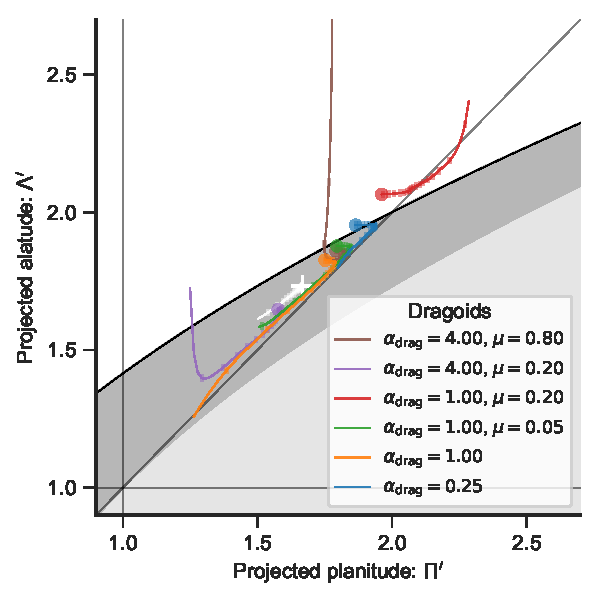
\includegraphics[width=\linewidth]{figs/dragoid-R90-vs-Rc}
  \caption{Diagnostic diagram for dragoids}
  \label{fig:dragoid-Rc-R90}
\end{figure}

%%% Local Variables:
%%% mode: latex
%%% TeX-master: "quadrics-bowshock"
%%% End:
